\subsection{Election November 8, 1960: *Kennedy vs Nixon}
\begin{frame}[t]{Election November 8, 1960: *John Fitzgerald Kennedy}
\small

\begin{columns}[T, onlytextwidth]
\column{0.48\textwidth}
\vspace{-1em}
{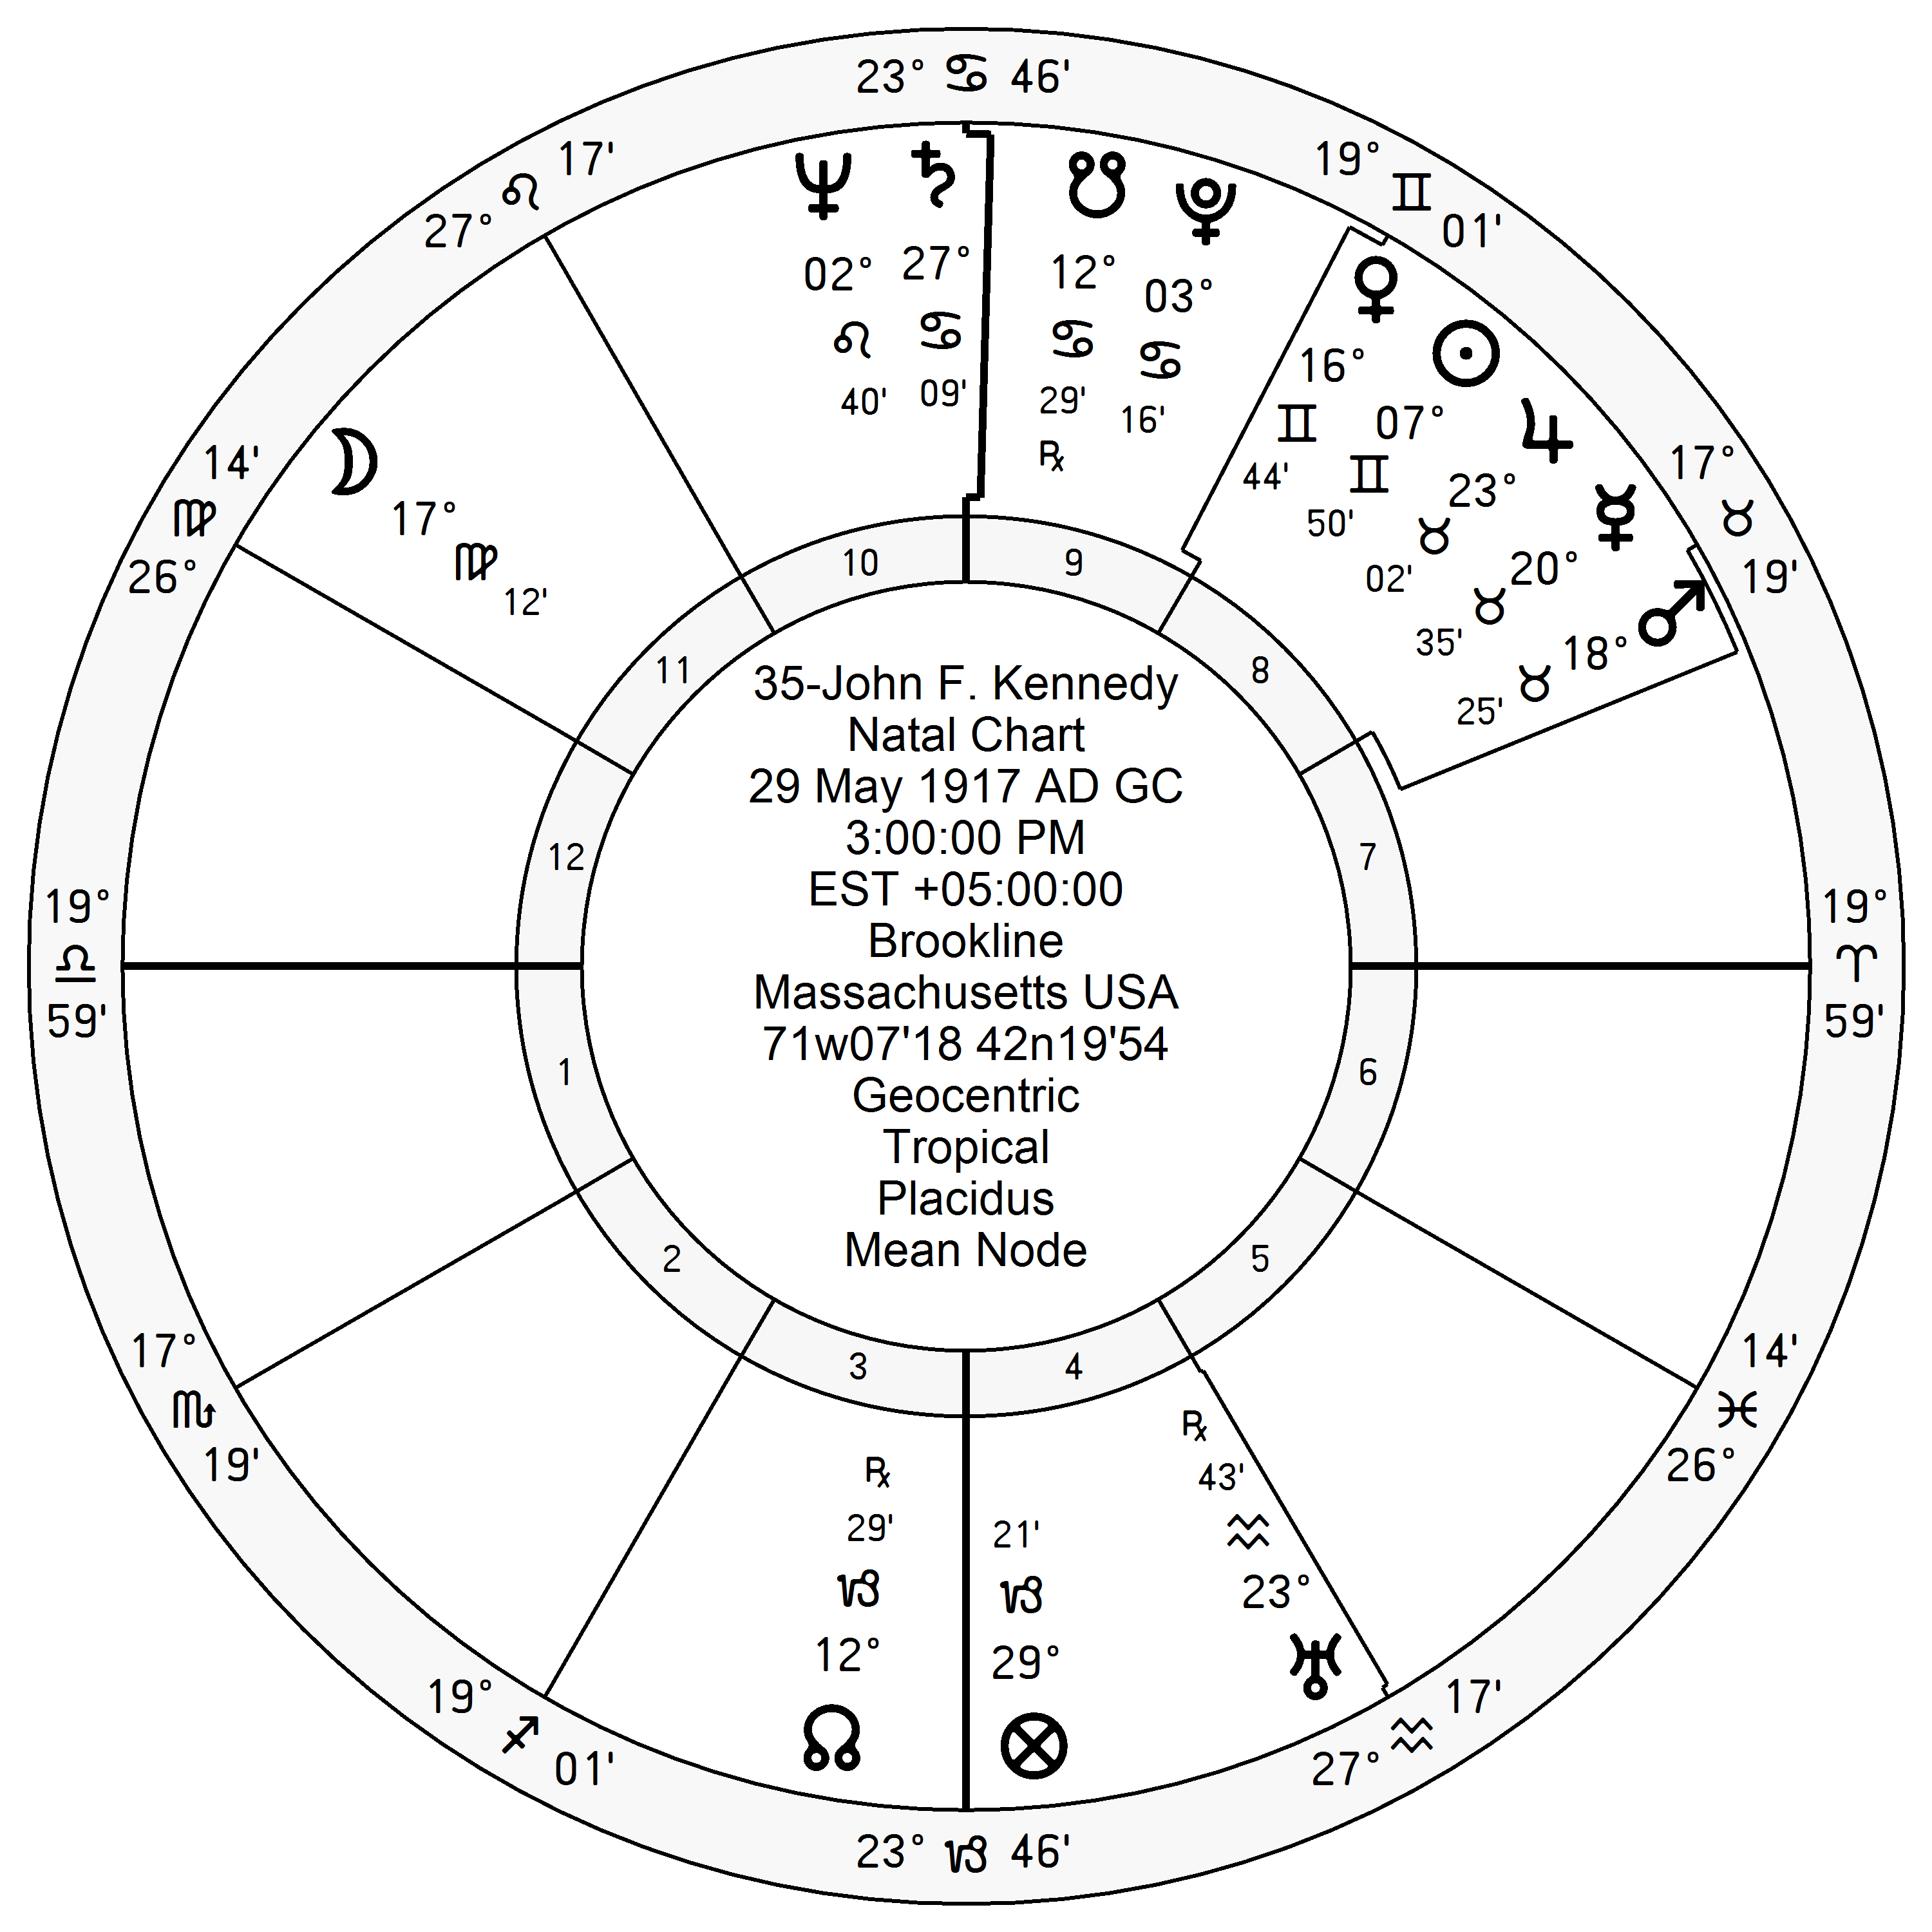
\includegraphics[width=0.9\textwidth]{charts/JFK.png}}
\fontsize{7pt}{8pt}\selectfont

\Venus\, (USB) in P1, \Square\, P10; \Sextile\, N10 \\
\Saturn\, \Sextile\, P1; in N10, \Square\, N1 \\
\vspace{0.5em}
The charts look weaker than Nixon's; possible Kennedy won because \Saturn\, as the exaltation ruler of the 1st, in the N10, with dispositor in the 11th `promises' a rise?


\column{0.48\textwidth}
\vspace{-1em}
{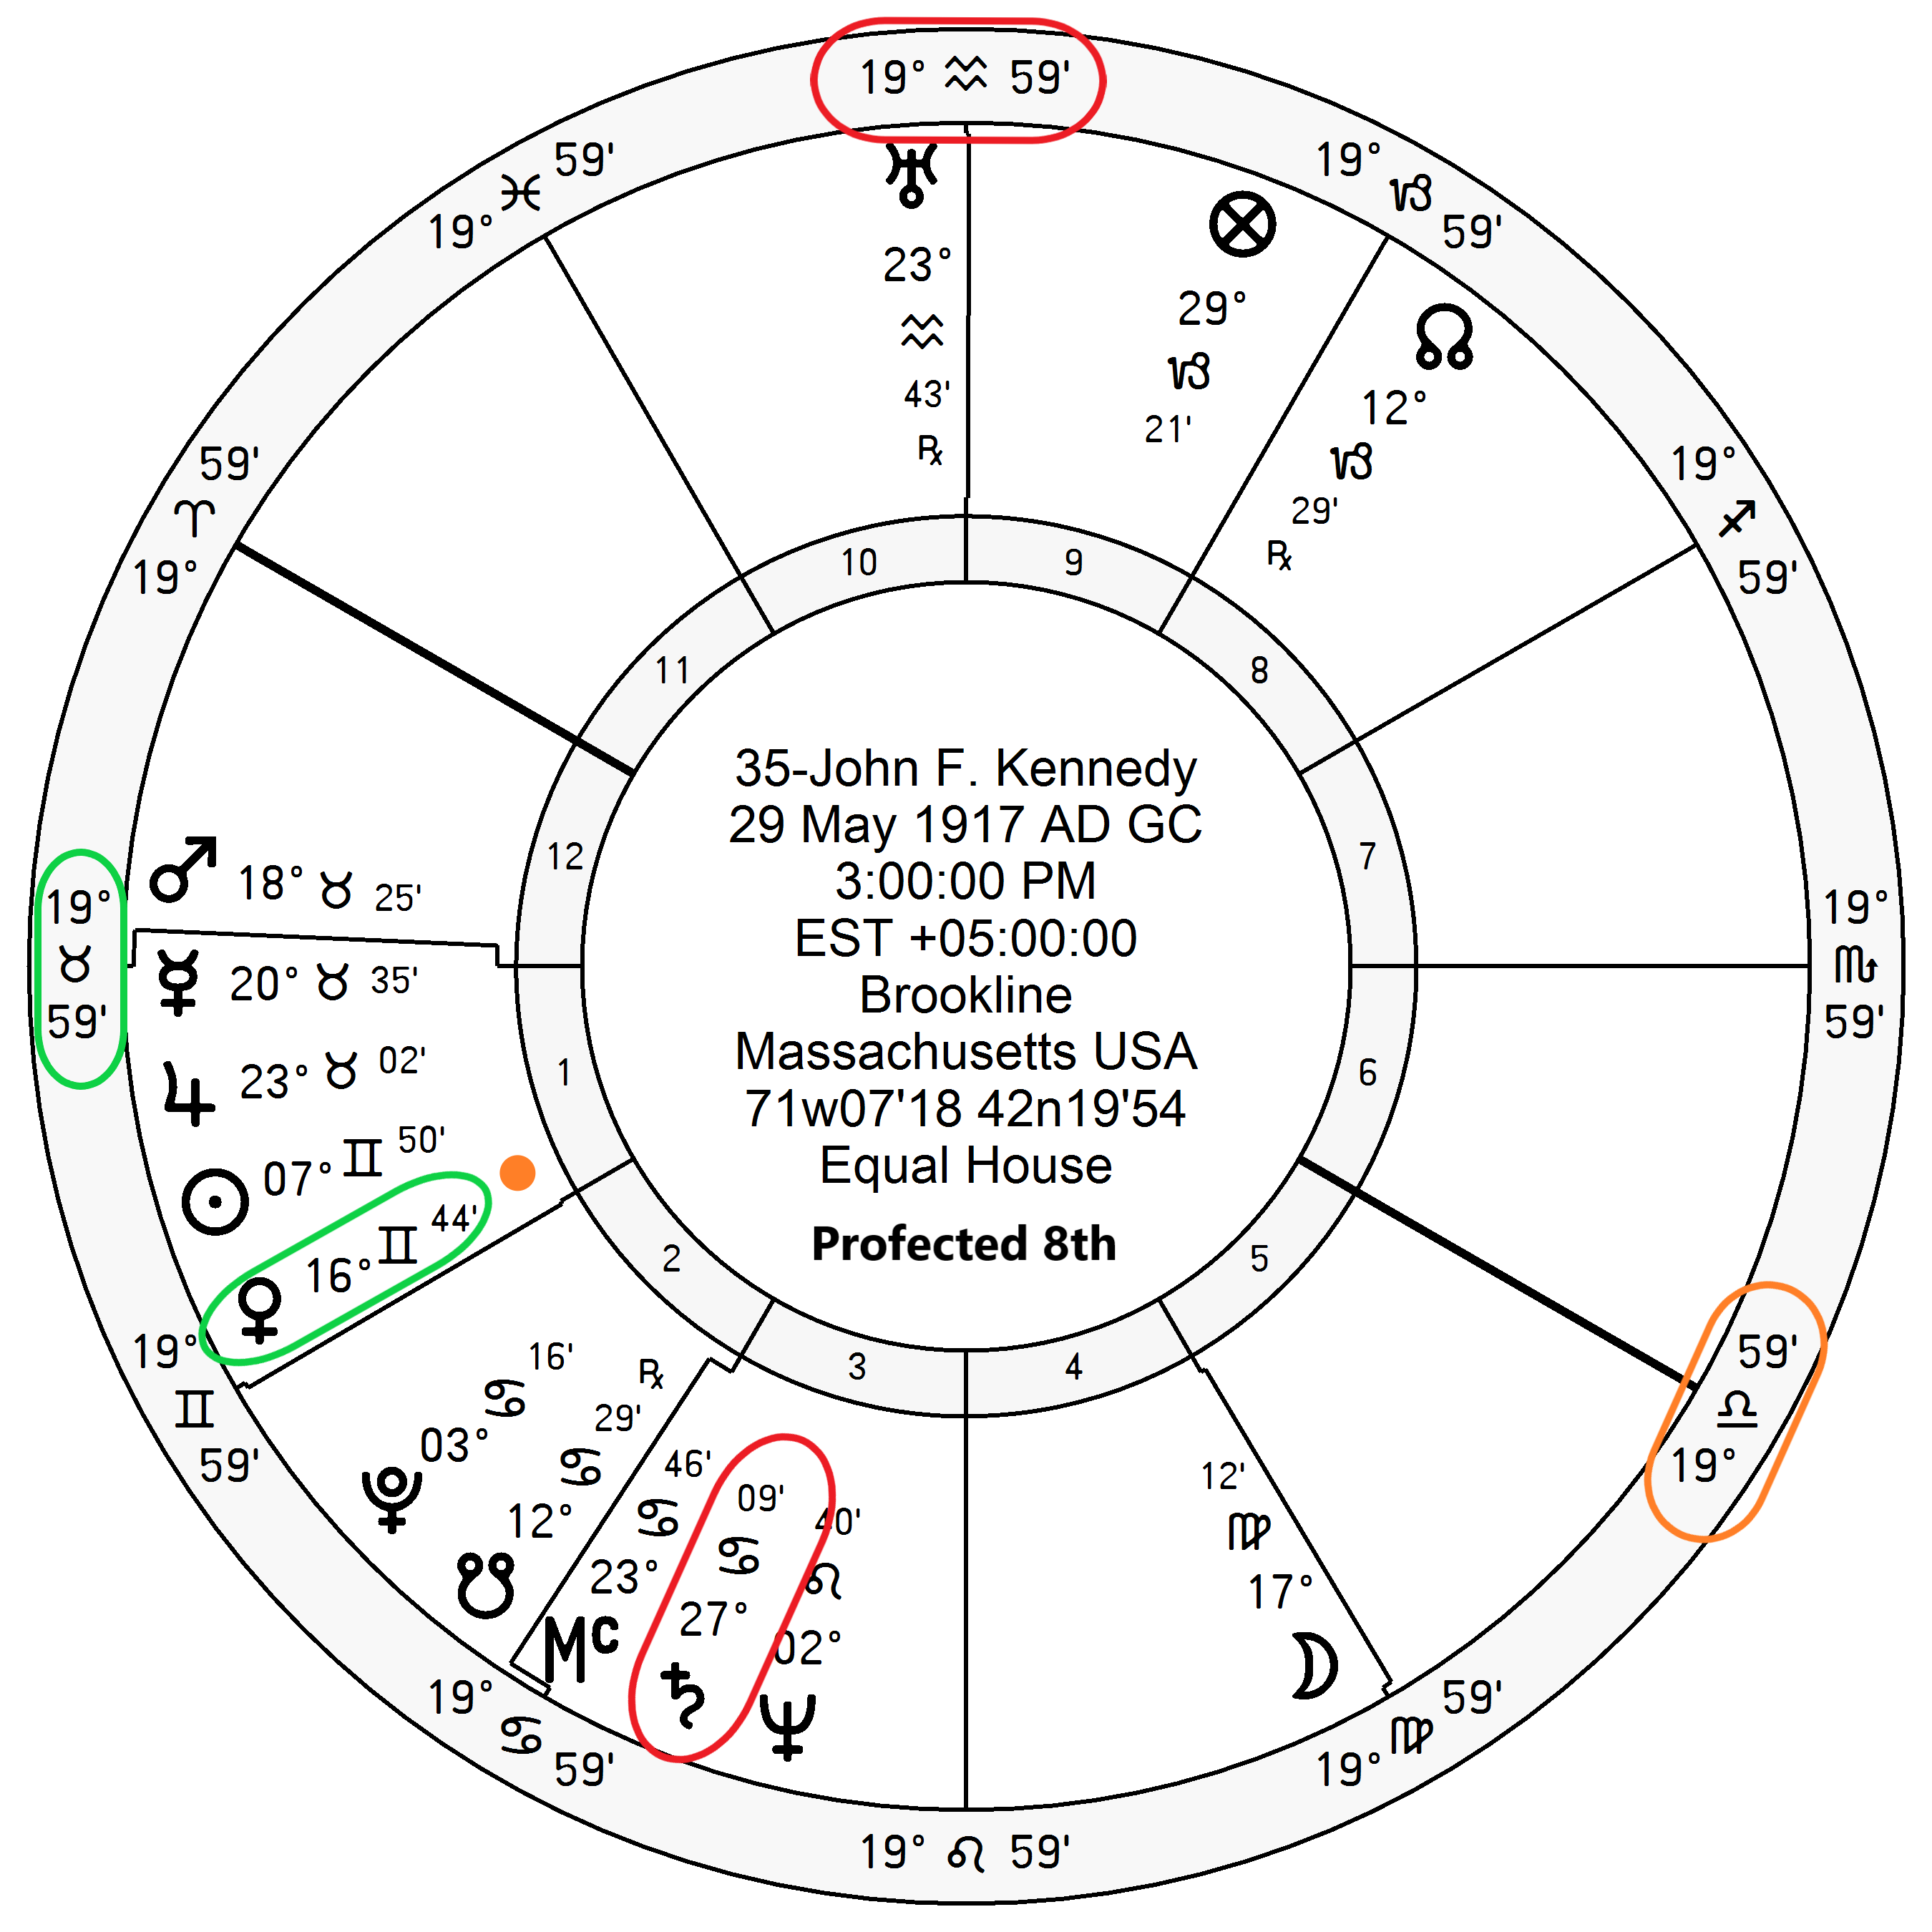
\includegraphics[width=0.9\textwidth]{charts/JFK-Prof-8th.png}}
\fontsize{7pt}{8pt}\selectfont

\textbf{\dgreen P1=N8}
	$\Rightarrow$ \Venus\, (USB) $\Rightarrow$ \textbf{\dgreen P1/N8} \\
\textbf{\red P10}=N5
	$\Rightarrow$  \Saturn\, $\Rightarrow$ P3/\textbf{\red N10} \\
PE=P6/\textbf{\dgreen N1}
	$\Rightarrow$  \Venus\, $\Rightarrow$   \textbf{\dgreen P1/N1}


\end{columns}
\end{frame}

% ===================================================
\begin{frame}[t]{Election November 8, 1960: Richard Nixon}
\small
\begin{columns}[T, onlytextwidth]
\column{0.48\textwidth}
\vspace{-1em}
{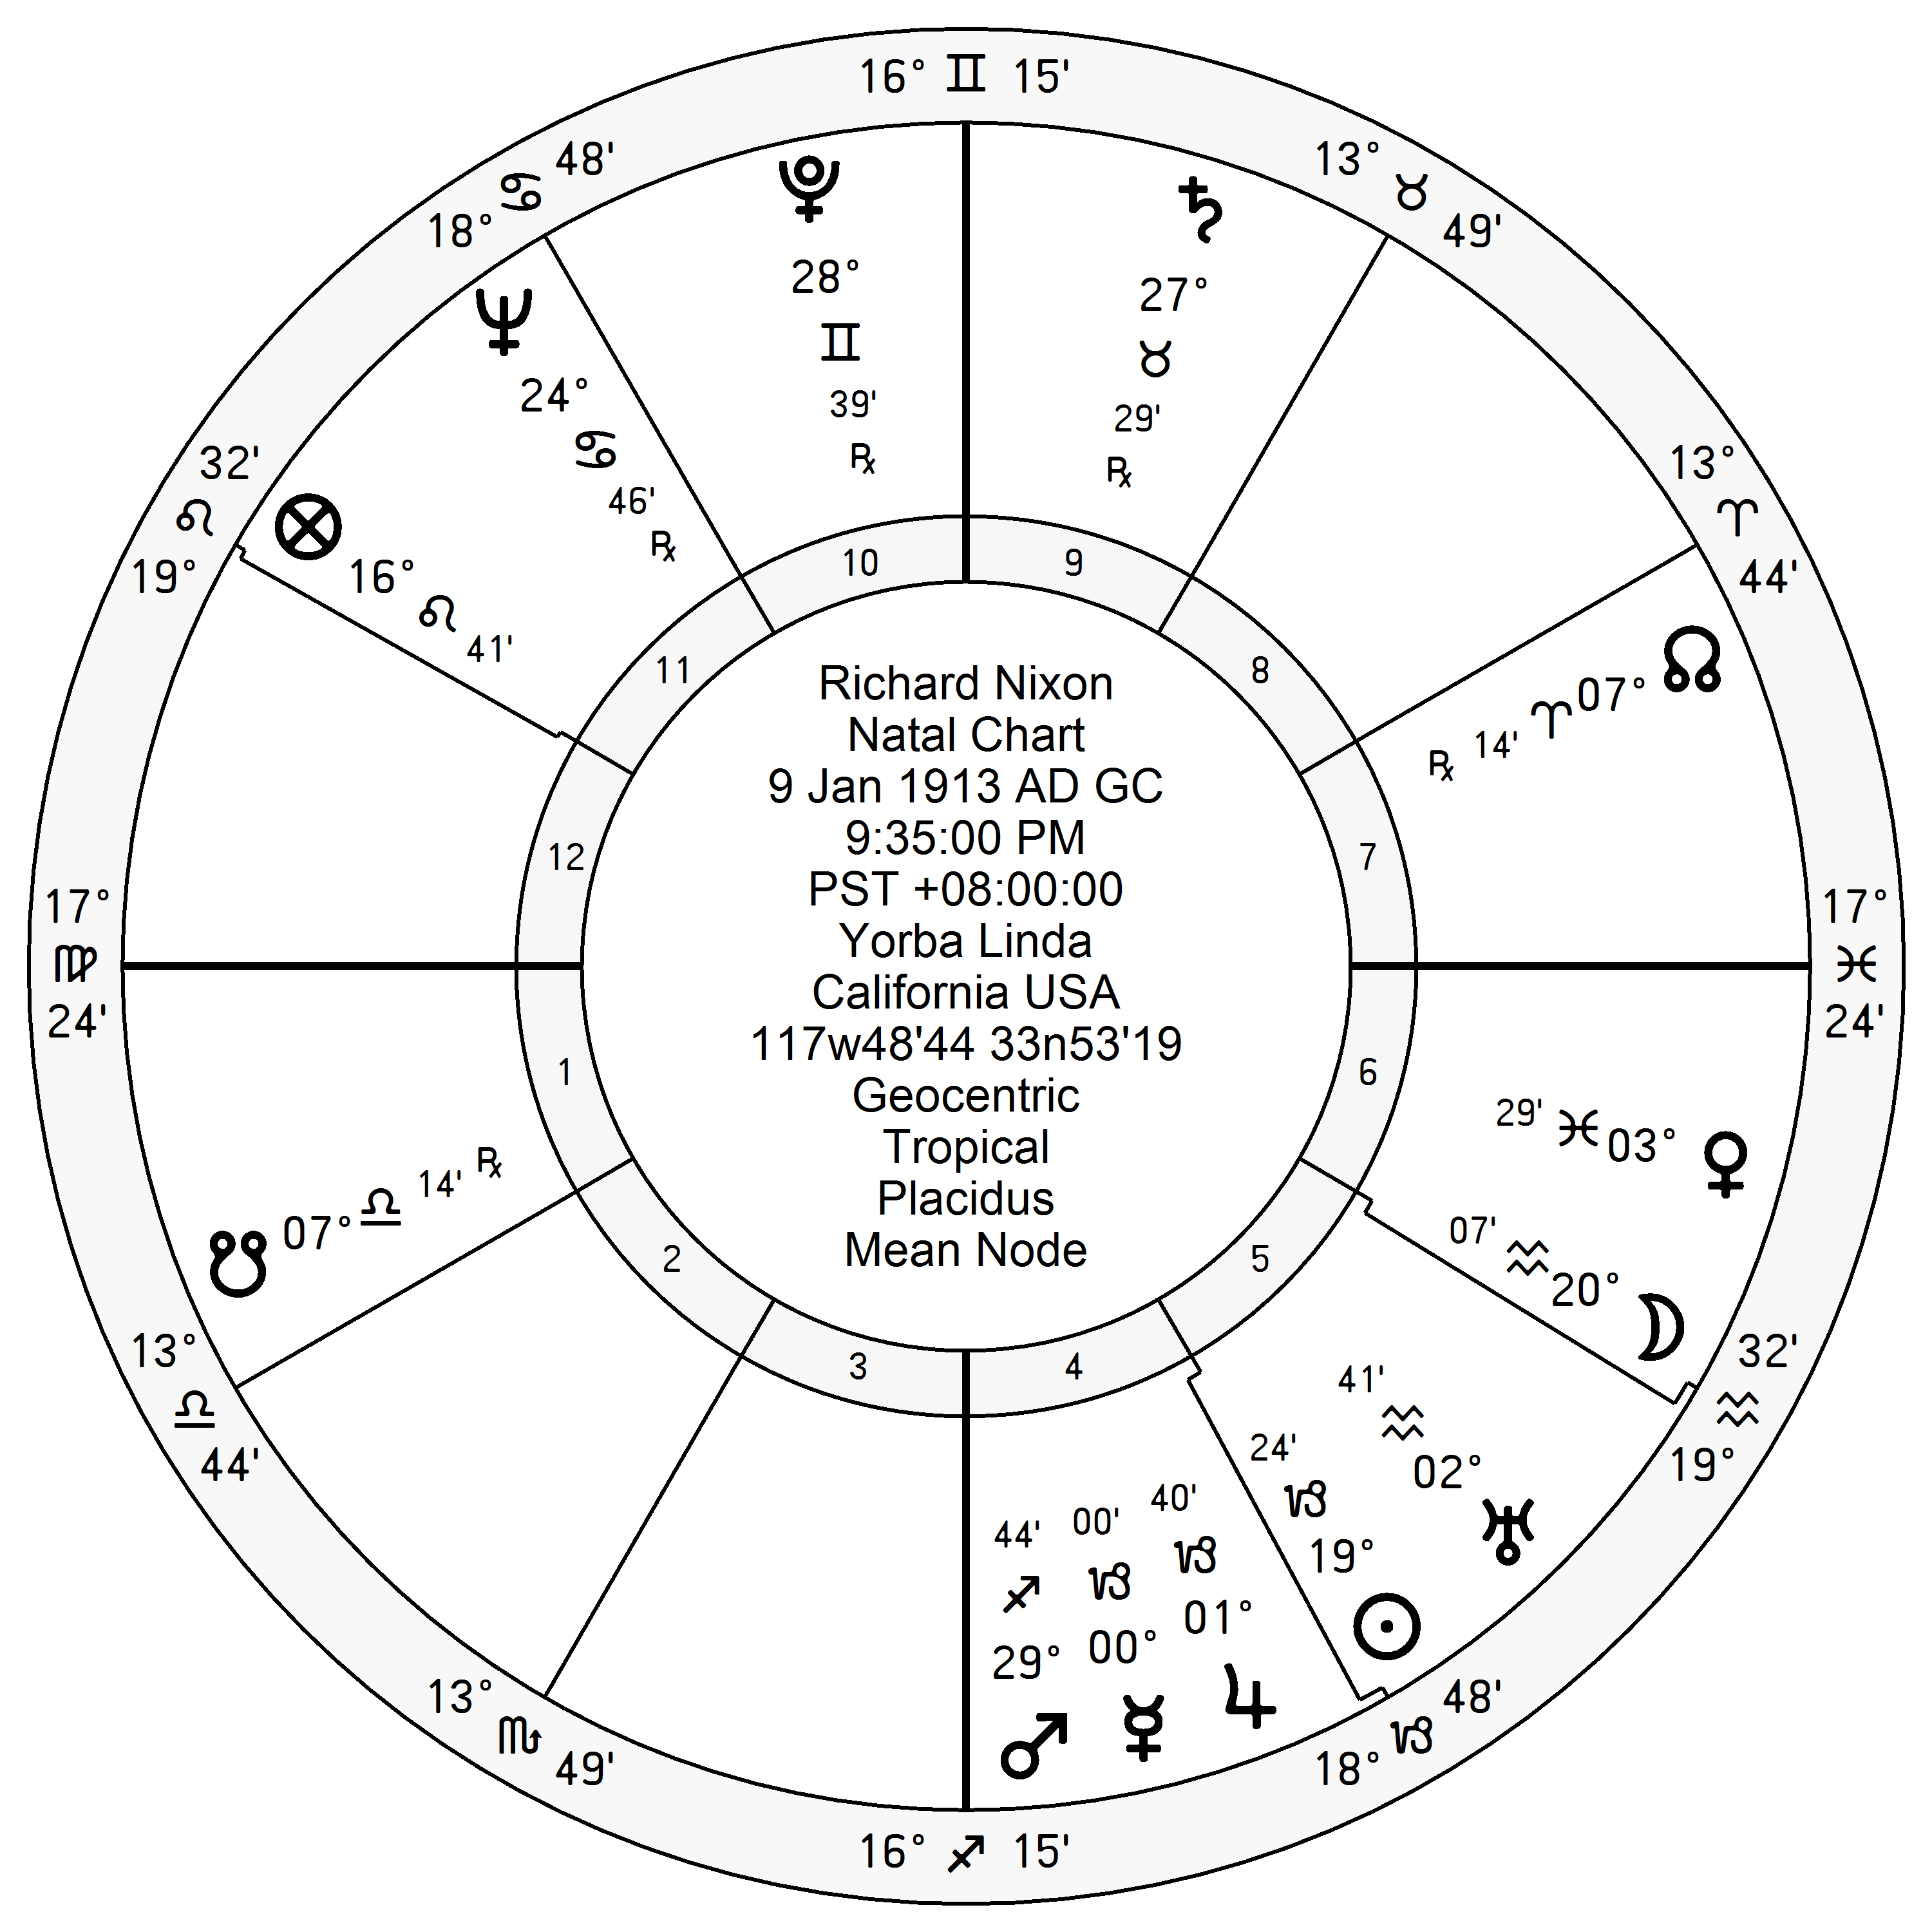
\includegraphics[width=0.9\textwidth]{charts/Nixon.png}}
\fontsize{7pt}{8pt}\selectfont

\Sun\, \Trine\, P10, \Trine\, N1 \\
\Venus\, \Square\, P10, \Opposition\, N1; \Trine\, N10 \\

\column{0.48\textwidth}
\vspace{-1em}
{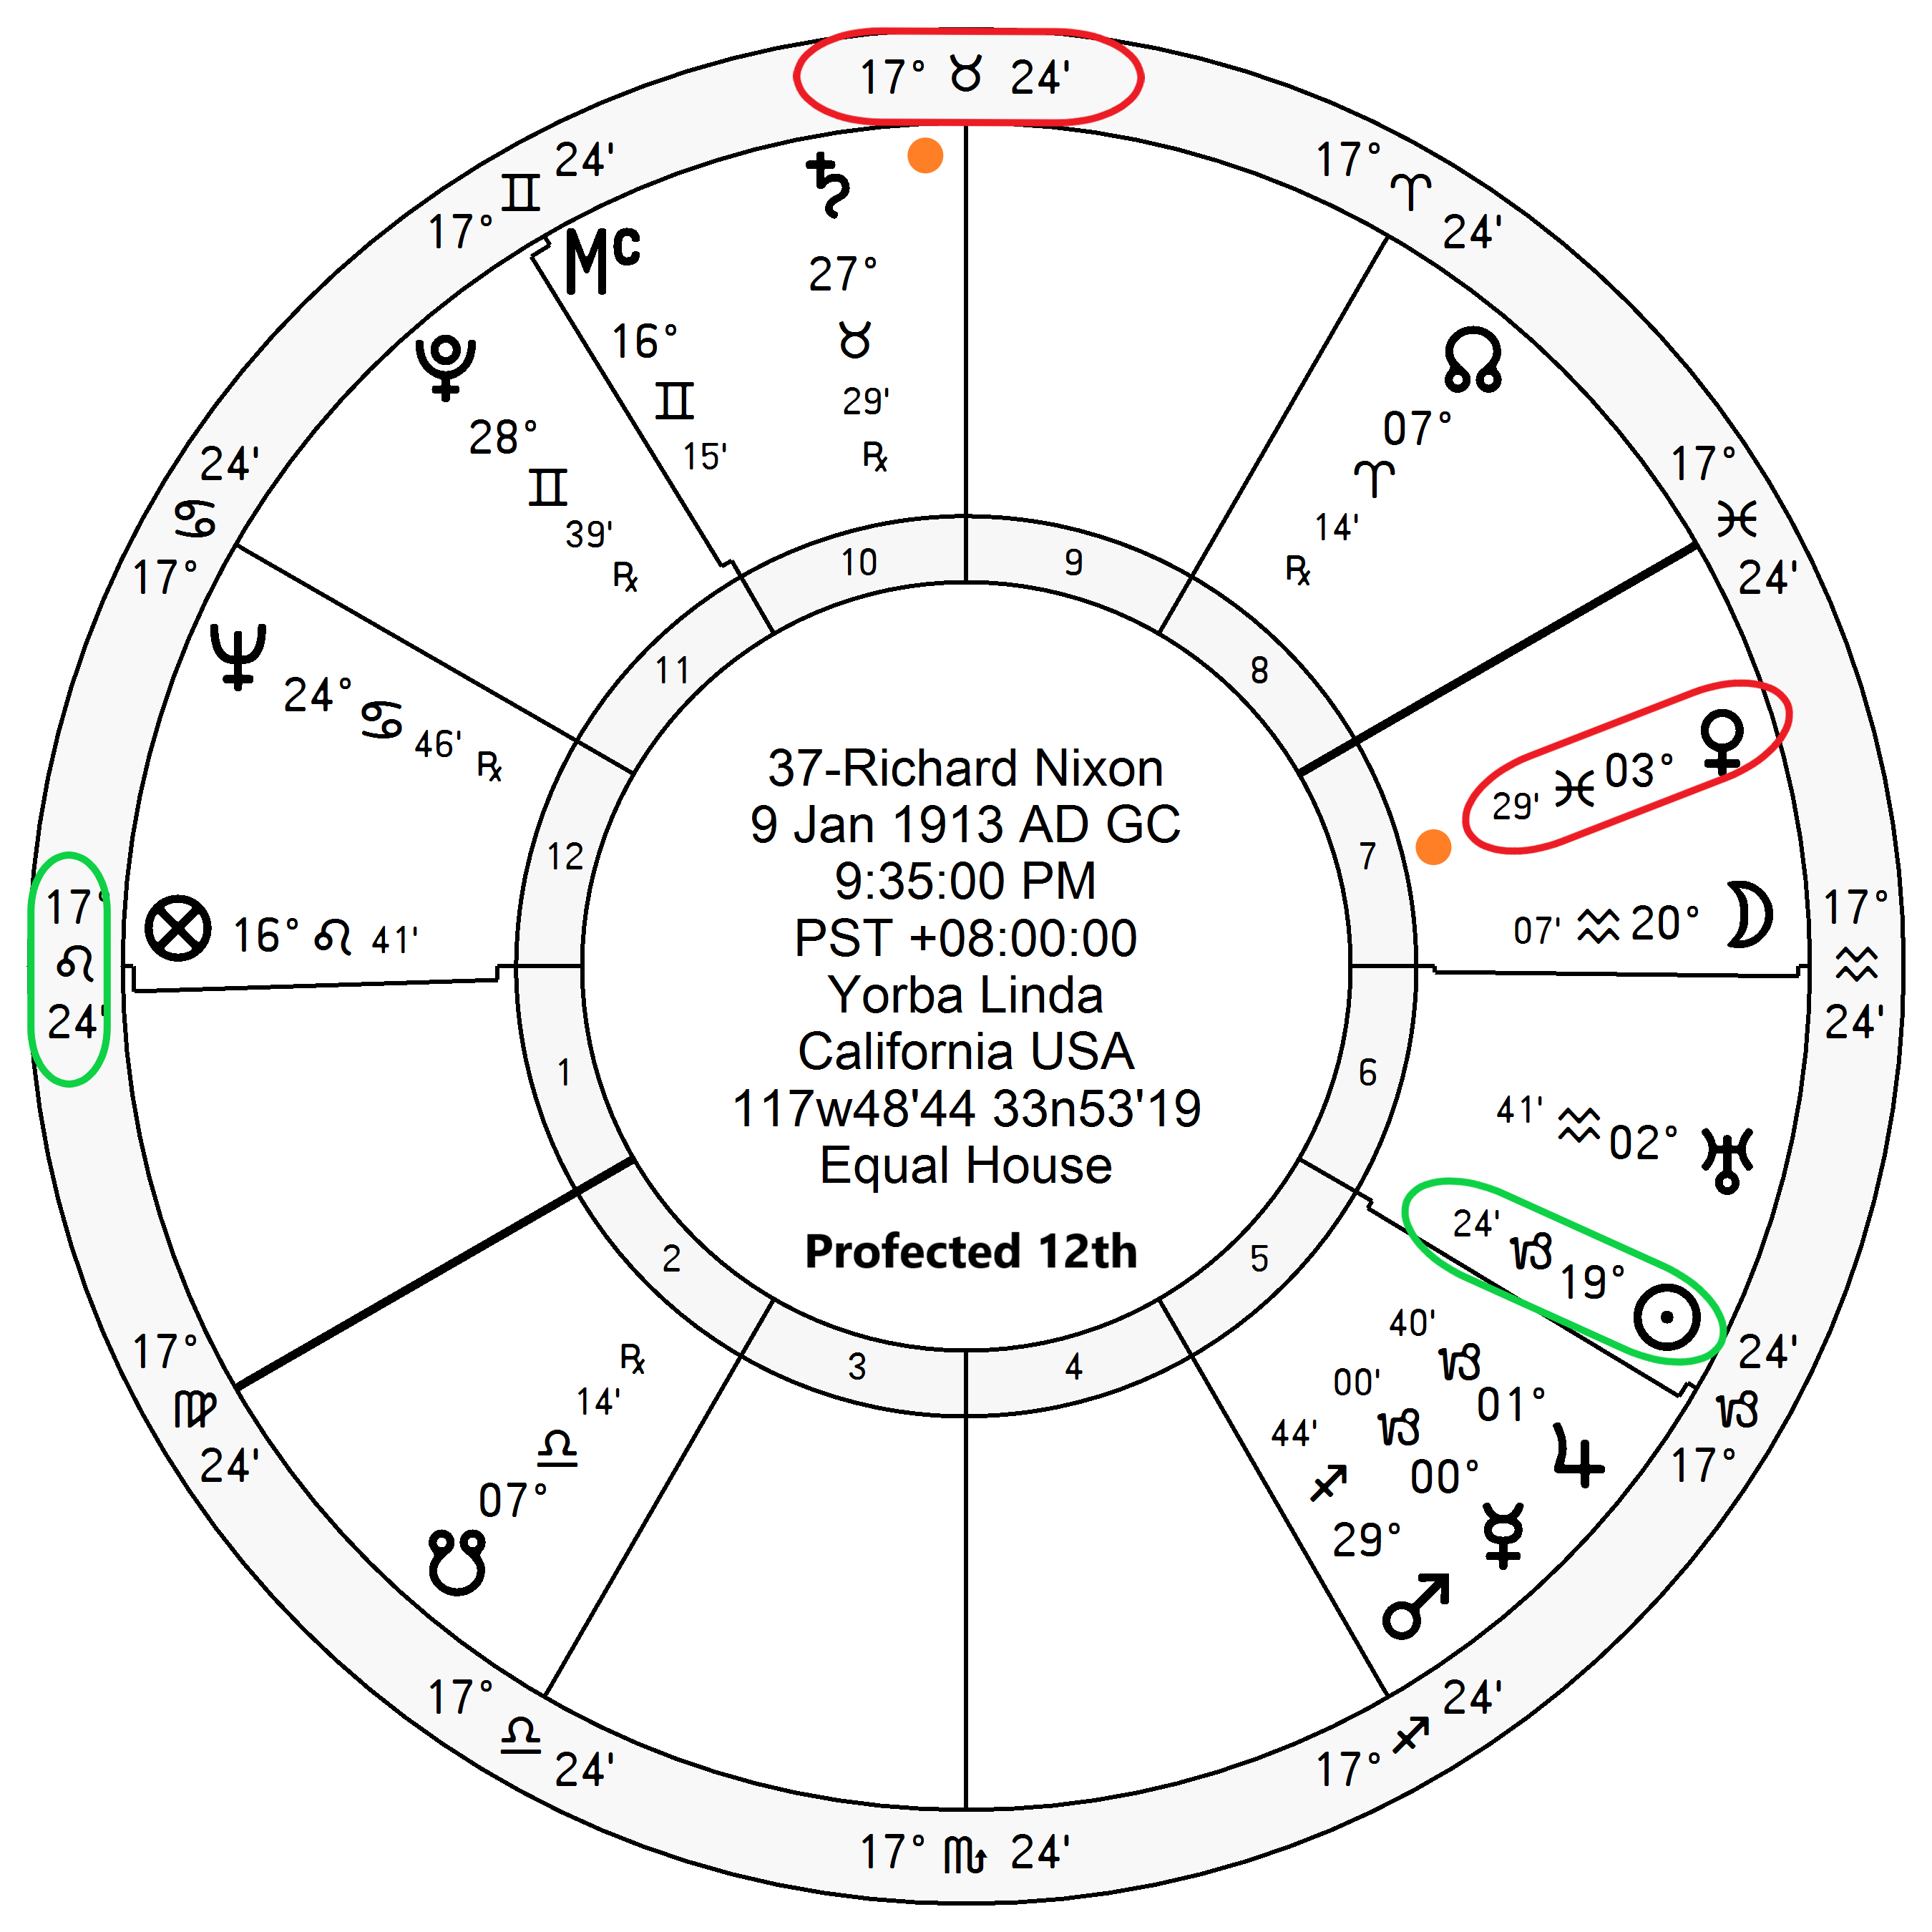
\includegraphics[width=0.9\textwidth]{charts/Nixon-Prof-12th.png}}
\fontsize{8pt}{9pt}\selectfont

\textbf{\dgreen P1=N12} 
	$\Rightarrow$ \Sun\, $\Rightarrow$ \textbf{\dgreen P6}/N5\\
\textbf{\red P10=N9}
	$\Rightarrow$ \Venus\, $\Rightarrow$ \textbf{\dgreen P7/N6}\\
PE=\textbf{\red P10/N9}
	 $\Rightarrow$ \Venus\, $\Rightarrow$ \textbf{\dgreen P7/N6}

\end{columns}
\end{frame}
